\documentclass{article}


% if you need to pass options to natbib, use, e.g.:
% \PassOptionsToPackage{numbers, compress}{natbib}
% before loading nips_2018

% ready for submission
% \usepackage{nips_2018}

% to compile a preprint version, e.g., for submission to arXiv, add
% add the [preprint] option:
\usepackage[final]{nips_2018}
\usepackage{fullpage}

% to compile a camera-ready version, add the [final] option, e.g.:
% \usepackage[final]{nips_2018}

% to avoid loading the natbib package, add option nonatbib:
% \usepackage[nonatbib]{nips_2018}

\usepackage[utf8]{inputenc} % allow utf-8 input
\usepackage[T1]{fontenc}    % use 8-bit T1 fonts
\usepackage{hyperref}       % hyperlinks
\usepackage{url}            % simple URL typesetting
\usepackage{booktabs}       % professional-quality tables
\usepackage{amsfonts}       % blackboard math symbols
\usepackage{amsmath}
\usepackage{nicefrac}       % compact symbols for 1/2, etc.
\usepackage{microtype}      % microtypography
\usepackage[pdftex]{graphicx}
\graphicspath{ {images/} }



\title{Reddit}

% The \author macro works with any number of authors. There are two
% commands used to separate the names and addresses of multiple
% authors: \And and \AND.
%
% Using \And between authors leaves it to LaTeX to determine where to
% break the lines. Using \AND forces a line break at that point. So,
% if LaTeX puts 3 of 4 authors names on the first line, and the last
% on the second line, try using \AND instead of \And before the third
% author name.

\author{
  Davide Spallaccini\thanks{\texttt{spallaccini.1642557@studenti.uniroma1.it}} \\
  Department of Computer, Control \\ and Management Engineering\\
  Sapienza University of Rome\\
  Rome, Italy \\
  \And
  Beatrice Bevilacqua\thanks{\texttt{bevilacqua.1645689@studenti.uniroma1.it}} \\
  Department of Computer, Control \\ and Management Engineering\\
  Sapienza University of Rome\\
  Rome, Italy \\
   \\
  %% examples of more authors
  \And
  Anxhelo Xhebraj\thanks{\texttt{xhebraj.1643777@studenti.uniroma1.it}} \\
  Department of Computer, Control \\ and Management Engineering\\
  Sapienza University of Rome\\
  Rome, Italy
  %% Affiliation \\
  %% Address \\
  %% \texttt{email} \\
  %% \AND
  %% Coauthor \\
  %% Affiliation \\
  %% Address \\
  %% \texttt{email} \\
  %% \And
  %% Coauthor \\
  %% Affiliation \\
  %% Address \\
  %% \texttt{email} \\
  %% \And
  %% Coauthor \\
  %% Affiliation \\
  %% Address \\
  %% \texttt{email} \\
}

\begin{document}
% \nipsfinalcopy is no longer used

\maketitle

\begin{abstract}

  Inspired by the "Community Interaction and Conflict on the Web"
  paper\footnote{Paper link}
  Machine learning techniques have been the driving component of research in
  many fields in recent years from advertisement, self-driving cars to
  healthcare. Although many models have been developed to improve accuracy
  performances it is often difficult to debug and understand them especially
\end{abstract}

\section{Introduction and Related Work}
\label{sec:intro}

Reddit is a growing social network based on communities called
subreddits where users interact by posting articles and links regarding
topics of the community and by commenting them. Interests of communities usually
overlap but the
opinions on the subject matter may diverge. In this context, a user of one
subreddit (source of the link) may post a cross-link (i.e. a link that
points to another subreddit which is the target of the link) and lead to
a mobilization where the users of the source community interact with the users
of the target community in the targeted post. The concept has been explored in
the paper "Community Interaction and Conflict on the Web" in which the authors
have constructed a dataset starting from 40 months of reddit content such as
posts and comments. The resulting dataset is composed of 394,216 instances of
mobilizing cross-links represented as id of source post, id of target post
and a label telling whether the mobilization was neutral/positive ("non-burst")
or negative ("burst").

Starting from the concept of user and community interactions on Reddit we
decided to reproduce some of the results of the paper to have an insight of the
process and understand the difficulties and challenges of the task. Based on the
dataset described above we applied a novel model employing deep learning
concepts,
using a combination of a convolutional neural network followed by an LSTM
recurrent network to predict whether a mobilization is positive or negative,
i.e. whether it will lead to a conflict. Additionally, on the target posts of
the negative mobilizations we analyzed the kinds of user-user interactions
developed by constructing a reply network of the comments for each post and 
applying personalized PageRank. Finally intrigued by the structure of the social
network we decided to find similarities between communities and construct a
recommender system to permit the users to discover new communities based on
their interaction history.

\section{Dataset Retrieval}
\label{sec:retrieval}

The "Community Interaction and Conflict on the Web" dataset is provided in a
preprocessed form where posts are represented by the indices of the word
embeddings of the words forming its title and body and users by a feature vector
that describes the activity levels and lexical features of their previous posts.
In order to have more flexibility over the design choices of our models we
decided to rely on that dataset only as a ground truth and to retrieve the raw
content from the source, i.e. the reddit social network. In particular we used
the Pushshift API in conjunction with the Python Reddit API Wrapper (PRAW). In
this task we encountered our first challenge which was due to the rate limiting
set by both the APIs which allow respectively an average of 120 requests and
60 requests per minute. Moreover to retrieve the necessary data for each
instance of the dataset multiple requests were required. By launching multiple
processes in parallel and using multiple accounts we were able to get the
most of the information needed.

For the LSTM-based classification task, given the post IDs of the sources of
the cross-links provided by the dataset, the Pushshift APIs were used to
retrieve: in a first request the text of the title and of the body of the post,
in a second one the ids of the top 8 comments present in the post and in a third
one the first 512 characters of the body of each comment to avoid giving too
much weight to the comments with respect to post text. The process just
described unfortunately incurred into some exceptions caused by rate limiting
and post deletion but still allowed to collect enough data for the
classification as will be described in Section \ref{sec:davide}.

To reproduce the analysis on the reply network we took only
the instances of the dataset that were labeled as "burst" i.e. the ones that
produced a negative mobilization. For each of the target posts we used the
PRAW library to retrieve its comments and the authors of those comments. Of the
authors, only the subset of users that were attackers or defenders were chosen.
In order to know whether a user is an attacker or defender we used the Pushshift
API to retrieve the comments submitted by the user in the 30 days before the
target post submission. An attacker (resp. defender) is a user who has made at
least one comment in the source (resp. target) subreddit in the 30 days prior to the
cross-link but who did not comment in the target (resp. source) during this time
period.

The gathering of the data for the subreddit similarities and the recommender
system was done by downloading all the comments submitted to reddit in December
2017. The data for each reddit month is available as a lmza compressed file at
\href{files.pushshift.io}{pushshift.io} in JSONLines format which is the
standard for Big Data. In this task we encountered another issue in dataset
retrieval since the size of the uncompressed file reached the size of $\approx
80$GB filling up the available disk space of the machine. We opted for first
performing a counting of comments by subreddit to spot the most active
subreddits represented in Figure \ref{fig:hist} by performing a scan over the
compressed dataset since lzma compression permits streaming decompression.

\begin{figure}[h]
\centering
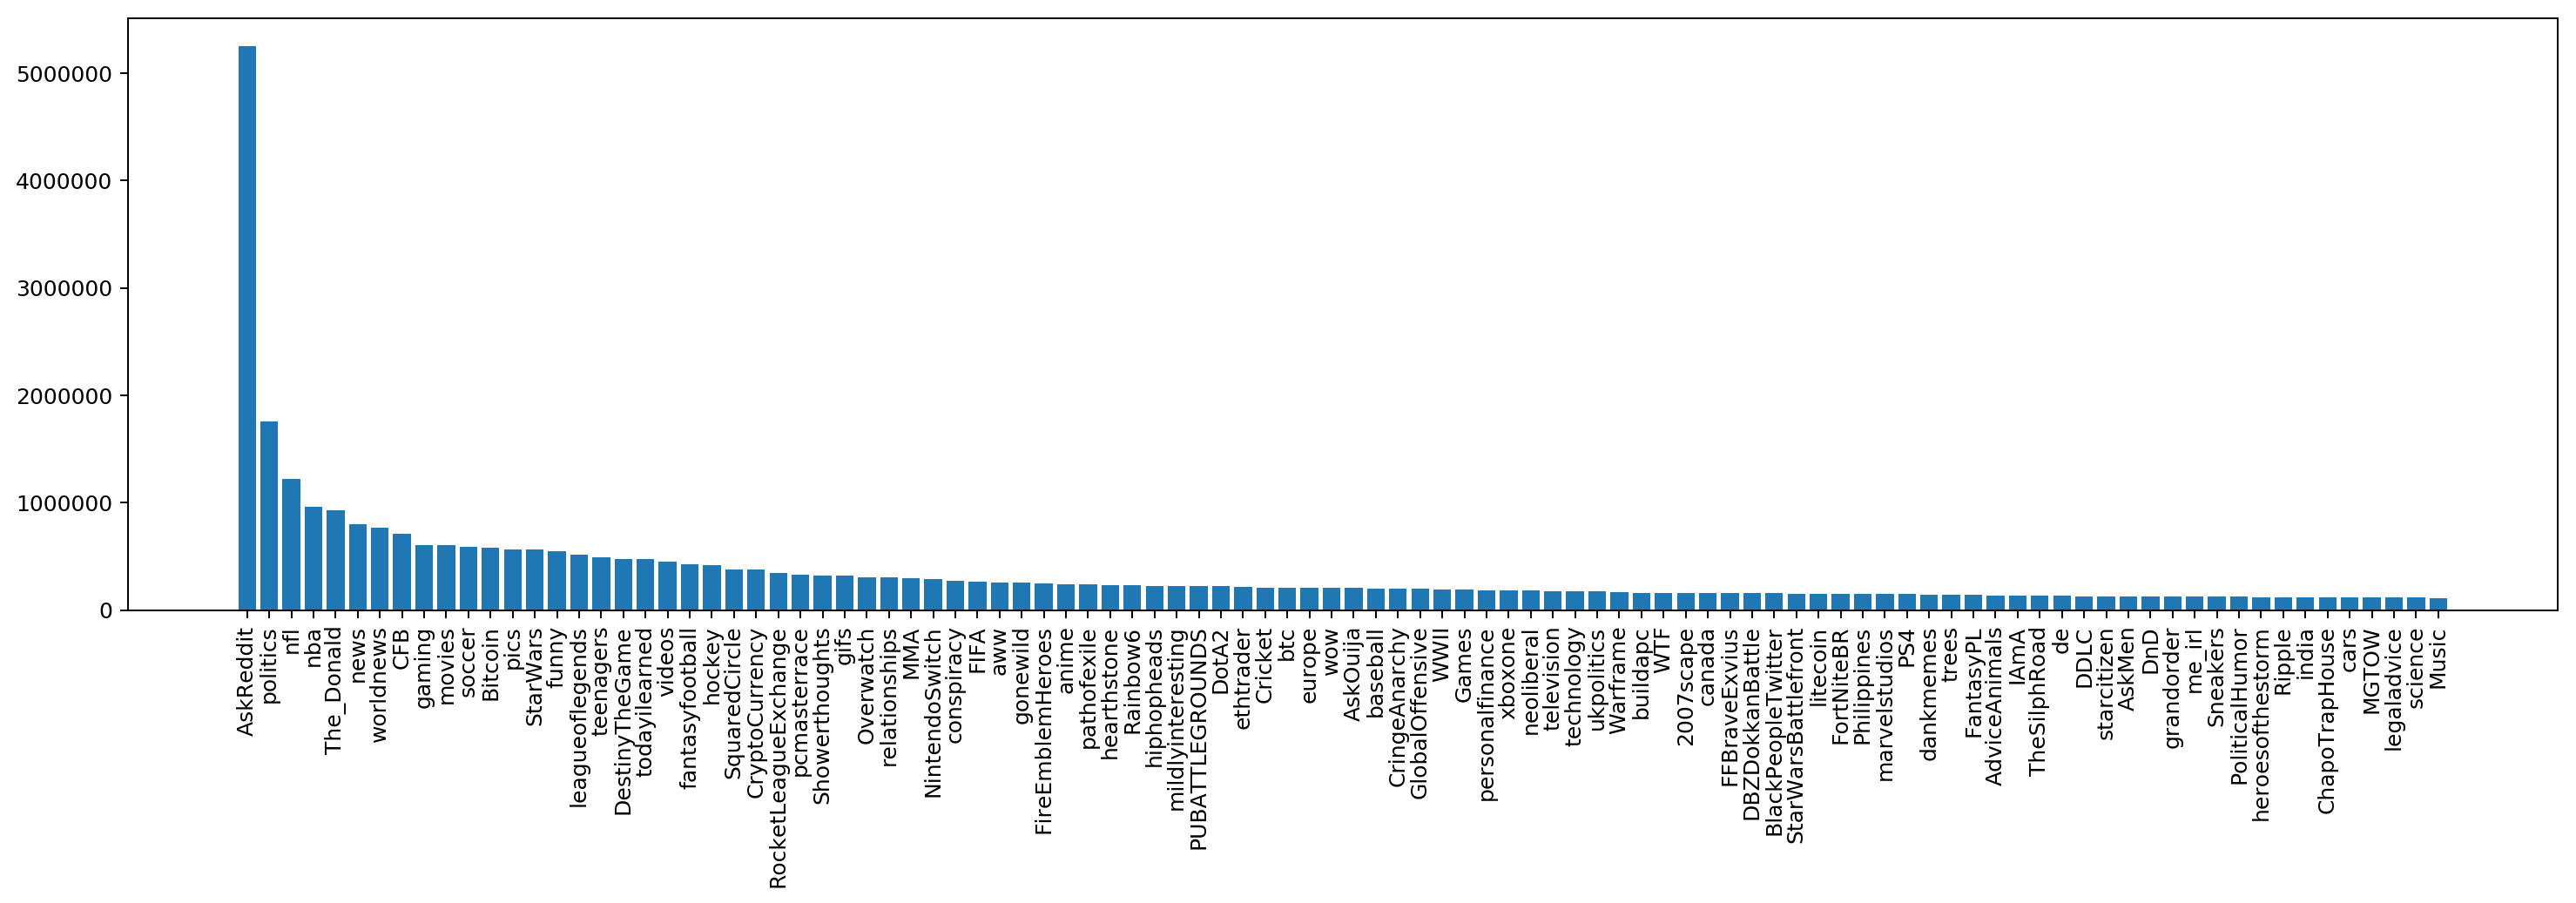
\includegraphics[width=\linewidth]{subreddit_activity.png} \\
\caption{Most active subreddits by number of comments in December 2017}
\label{fig:hist}
\end{figure}

Since processing such dataset was unfeasible on a standard desktop we decided to
take a sample of it by keeping each comment in the original dataset with a
probability of $\frac{1}{4}$ and transforming the format from JSONLine to csv
which reduces the space needed for storage.


\section{Mobilization Sentiment Prediction through LSTM}
\label{sec:davide}

The author's dataset was built with the help of Mechanical Turk crowdworkers
that manually annotated almost a thousand of cross-links telling whether the
sentiment of the source post towards the target post was negative or
positive/neutral reaching a inter-rater agreement of 0.95. Over this sample the
authors applied a Random Forest classifier with forests of 400 trees that
achieves an accuracy of 0.80 on a 10-fold cross validation. They then used this
classifier to build the dataset presented in Section \ref{sec:intro}. Such
dataset was used as a ground
truth to train our model. By performing the retrieval described above we
obtained a set of instances of which about 95\% labeled as positive as
announced in the original paper raising another challenge. Such unbalancing
between the number of
instances of the classes would produce an unreliable evaluation therefore we
chose to undersample the retrieved dataset. Instead of using a random heuristic
we used the NearMiss version 1 method that reduces the number of positive
elements by keeping only those positive instances for which the average distance
to the N closest samples of the negative class is the smallest. After
undersampling we obtain a dataset of about 8,000 instances that is split into
80\% of training set and 20\% of test set.

Instead of employing the large set of features, that by the way are not
very well documented, used by the authors in this setting we propose an improved
model based on the bare content of the post and its comments in terms of
contained words. This is a trend in modern classification methods
where deep learning models substitute annoying feature engineering.


Our model is essentially based on a combination of a convolutional
neural network followed by a LSTM recurrent network. At the basis of the model we
use GloVe word embeddings that allow us to represent each word in the text in a fixed-
size, compact and dense vector of 300 floats also taking into account similarity between
words. The advantage of GloVe vectors over the simple one-hot representation of words
is that these vectors were trained using a neural network so that words that have a
similar context are close in the vector space. Then the word embeddings are given in 
input to the convolutional layer. The purpose
of this layer is to capture more general patterns in the data helping the network to better
generalize to new examples without excessively specialising on the text of the training
data. The result is given in input to the bidirectional LSTM layer which is responsible
of learning the patterns in the sequences of words, something that recurrent network
were designed to do well. In particular the LSTM architecture allows to ”remember”
longer sequences learning which parts of the sequences are more important. After
some tuning of the hyperparameters we obtained a classifier with the following
performances.

\begin{verbatim}
             precision    recall  f1-score   support

  non-burst       0.87      0.93      0.90       769
      burst       0.93      0.87      0.90       807

  avg/total       0.90      0.90      0.90      1576
\end{verbatim}

\section{Attacker Defender PageRank}

To understand whether in the target post of a negative mobilization attackers
and defenders talk to each other or they form their own groups thus creating
echo chambers we construct a graph of the users' interactions.
In fact, reddit
comments can be nested and a comment can be in response to another comment.
From this scheme, a reply network is
constructed where each node is a user, either attacker or defender, and a
directed edge from user $i$ to user $j$
indicates that $i$ replied to one of $j$'s comment. The weight of the edge
indicates the number of times a user replied.

We quantify the echo chamber by replicating the approach of the paper which is
based in the application of personalized PageRank: firstly by restricting the
teleport set to the defender nodes (Defender PageRank) and secondly to the
attacker nodes (Attacker PageRank). The Defender PageRank (resp. Attacker
PageRank) score of a node represents its centrality measured from the perspective
of Defender nodes (resp. Attacker nodes).


\section{Recommender System}

Interested in the properties of the reddit social network, we decided to extend
the analysis provided in the reference paper by trying to implement a
subreddit recommender system. In order
to implement such system we preferred to not perform a crawl of the reddit
website since it could have produced a bias in the result coming from the fact
that the communities are not necessarily linked. Instead we chose to use the
sample of the reddit comments of December 2017 retrieved as explained in Section
\ref{sec:retrieval}. This is of course an over-semplification of the task but it
is based in the often valid assumption that contents of subreddits do not change
rapidly at the granularity of the month.

The first phase of the design process was to choose how to tackle the problem.
We thought about experimenting a Collaborative Filtering approach but the amount
of users in the sample and the sparsity of user-subreddit matrix would have not
been significantly effective. Instead we opted for a Content-Based system using
subreddit similarities. We decided to represent a subreddit as the TF-IDF vector
of the most frequent words in its comments. We split the computation into
multiple phases. In the first phase we grouped comments by subreddit. In the
second phase we tokenized the comments, removed stop words and performed
stemming based on the Porter algorithm. Finally we computed the TF-IDF vector of
length 10,000 for each subreddit by considering a vocabulary with the 10,000
terms having the highest TF.

To qualitatively test this representation of subreddits we decided to compute
the most similar subreddit for each subreddit. Indeed we've found out
similarities between subreddits about sports, news, funny posts etc.

To evaluate

\iffalse
Several papers have been published based on the Wisconsin Breast Cancer
Diagnostic (WBCD) dataset of which main challenge is to provide an outstanding
classification of patients given their Fine Needle Aspiration (FNA) attributes
to detect whether the nuclei will develop into malign or benign cancer. The
dataset was created by Dr. W. H. Wolberg using fluid samples of the masses and
applying graphical tools to compute ten features from each of the cells of the
sample to then calculate their mean value, worst value and their standard error
returning a 30 real-valued vector for each patient. The dataset contains 569
instances of which 357 labeled as benign and 212 malign.

\begin{figure}[h]
\centering
\includegraphics[width=0.4\linewidth]{masses.png} \\
\caption{Line fitting of the nuclei extracted through FNA to compute features}
\end{figure}
The importance of the task comes from the fact that the main techniques applied
for Breast Cancer detection are based on visual interpretations of mammographies
and FNAs or surgical biopsy. While the latter is more accurate, it is also the
most expensive and invasive. Machine learning techniques applied to the former
are helpful since allow to speed up and partially automate the analysis of
patients but we cannot rely on machine learning alone in such critical tasks
since it can produce alarming false positives and unexplainable results.

In order to merge the helpfulness of machine learning and the need of
explanations we developed Surfboard, a visual dashboard that permits not only to
classify a new patient based on previous experience given by the dataset but
also explore the data, to focus on interesting subsets of it, discover
similarities between patients and to find
discriminative features.

The values of the attributes are dimensionless numbers derived from the
graphical tool as function of cell characteristics in the image such as: number
of pixels occupied by a cell, intensity of colors, regularity of shape etc.


\section{Decision Tree Learning}

Decision Trees are a widely used predictive model that given a dataset, its
attributes and a target attribute tries to build a model that predicts the
target value of a new instance. Differently from other models it is not based on
optimizations of objective functions, instead a tree is built where each
internal node is a predicate over an attribute's value and each edge is a
possible outcome of the predicate at its upper node. The leaves of the tree are
 possible classification values.

In this scenario classifying a new instance reduces to following a path of the
tree from root to leaf testing at each level the given attribute and following
the edge corresponding to the outcome of the test.

In order to construct the tree we need to define an heuristic by which to 
choose the attributes to test at each step.
The chosen heuristic is fundamental since it constrains
the model only to a subset of possible topologies and thus its flexibility.

One approach of tree construction is to select at each step the attribute that
provides the highest \emph{Information Gain} which is measured as expected
reduction in \emph{Entropy} caused by knowing the outcome of the predicate over
the attribute. The entropy $E$ of a set $S$ of instances where the
target attribute can be either positive ($\oplus$) or negative ($\ominus$) is defined as:

\[ E(S) = -p_{\oplus} \log_2 p_{\oplus} -p_{\ominus} \log_2 p_{\ominus} \]

Where $p_{\oplus}$ is the portion of instances labeled as positive and
$p_{\ominus}$ as negative in $S$. In case the set contains instances of only
one class the entropy equals 0, while if the instances of the two classes are
equally distributed it is equal to the highest value possible, i.e. 1. If there
exist some predicate over an attribute $A$ such that the set $S$ is partitioned
into two subsets $S_1, S_2$ with $E(S_1) = 0$ and $E(S_2) = 0$, i.e. each
partition contains only instances of one class then attribute $A$ is a relevant
attribute for the classification since it allows to determine the target value
of instances. Following this reasoning at each step the attribute chosen is the
one having the highest information gain defined as:

\[ Gain(S, A) = E(S) - \sum_{v \in predicate(A)} \frac{|S_v|}{|S|} E(S_v) \]

Where $v \in predicate(A)$ is the outcome of the predicate which can be either
true or false and $S_v$ is the set of instances in $S$ having the outcome of the
predicate equal to $v$.

Decision trees have been extensively applied to classify medical patients
since they can provide intuitive, attribute-driven explanations. By applying the
CART algorithm with the expected Entropy reduction criterion to our dataset we
get a tree of which prefix is presented in Figure \ref{fig:tree}. The model
achieves an accuracy of $91.23\%$.

\subsection{Parallel Coordinates by Tree Learning}
\label{sec:treelearn}


Although very powerful, Decision Trees are highly dependent on the data and
using them as a black-box does not result into a robust diagnosis. Instead, we
can use the information captured by the learning algorithm and display it to the
user in order let the expert in charge to evaluate whether there is a strong
discriminative factor inducing a confident diagnosis or whether there is a need
to further investigate the case.

Moreover Decision Trees may result cumbersome to interpret and require further
data analysis to understand its structure and predicates.

Alternatively by visualizing the most relevant attributes discovered by the Tree
model we capture the essence of the information extracted by the learning
algorithm and permit the user to deduce himself the predicates and the main
characteristics of such attributes. Indeed as can be seen in Figure
\ref{fig:parallel} the threshold values discovered by the Tree are easily
distinguishable in the parallel coordinates.



\begin{figure}
\centering
\includegraphics[width=\linewidth]{tree_high.png} \\
\caption{Output of the Decision Tree built by applying CART to the WBCD
dataset with Entropy criterion. The hue of the color represents the entropy of
the dataset at a given node and the change in hue from parent to children
represents the expected reduction in entropy obtained by choosing that
attribute, i.e. its information gain.
Three attributes that allow to easily discriminate between
the two classes are highlighted.}
\label{fig:tree}
\end{figure}



\begin{figure}
\centering
\includegraphics[width=\linewidth]{parallel_coordinates_high.png} \\
\caption{View of the Surfboard tool where six features
    having the highest \emph{Gini score} (function of Information Gain
    considering the whole tree) are represented in the parallel coordinates
and the score for each feature is encoded in the bar chart in the lower right.
The attributes are represented by decreasing score from left to right.
As can be seen the values highlighted in the Decision Tree are neatly visible
in the parallel coordinates chart.}
\label{fig:parallel}
\end{figure}


\section{Linear SVM Classification}

A performant classification algorithm for high dimensional data is Support
Vector Machines (SVM) which is based on solving an optimization problem to find
the hyperplane that best separates the instances of different classes.
SVM is based on the vector space model in which each instance of the dataset
is represented as a vector in a high dimensional space which is defined
by attributes' domains. The output of the
optimization problem is a linear discriminant function $f(\mathbf{x})$
that given in input an instance $\mathbf{x}$ produces as result a scalar of
which sign represents the classification and absolute value represents the
distance from the hyperplane defined by the function.

If we map the two possible values of the classes to $t \in \{-1, 1\}$ 
the optimization problem solved is

\begin{equation}
    \begin{split}
        & \min_ {\mathbf{w}, b, \zeta} \frac{1}{2} \mathbf{w}^T \mathbf{w} + C
\sum_{i=1}^{n} \zeta_i\\
\textrm{subject to } & t_i(\mathbf{w}^T \mathbf{x}_i + b) \geq 1 - \zeta_i,\\
                       & \zeta_i \geq 0, i=1, ..., n
\end{split}
\end{equation}

Where $\zeta_i$ is a tolerance factor to misclassifications, $C$ a constant
representing the cost of the misclassification, $\mathbf{x}_i$ is the $i$-th
instance of the dataset and $t_i$ its target value.

The optimization problem tries not only to give a correct classification of the
dataset but also to maximize the distance of the hyperplane from the two
classes (large margin principle). The points that lie on or beyond the boundary
of their class are called support vectors and are the points that allow to
determine the hyperplane.


\begin{figure}[h]
\centering
\includegraphics[width=0.7\linewidth]{supports.png} \\
\caption{Intuition of SVM applied to two dimensional dataset.}
\label{fig:supports}
\end{figure}

\subsection{Visualizing the hyperplane through PCA}
\label{subsec:pcahyp}

In Surfboard we included the Linear SVM classification model which achieves an
accuracy of $93.61\%$. The user can insert the values of a new patient to be
classified by the tool. To better evaluate the output of the classifier
and have a grasp of the confidence in the classification of the new instance,
its vector is projected into a 2D PCA scatterplot computed from the dataset.

While with two dimensional datasets it is easy to visualize the hyperplane found
by SVM since it is just a straight line, this cannot be done with higher
dimensional data since the projection of the hyperplane on the dimensions found
by PCA can result into the whole plane defined by PCA itself.

To overcome this issue and still provide to the user a sense of distance of the
hyperplane from the instances of the classes, support vectors are highlighted in
the scatter plot PCA projection with the additional information of misclassified
points.

In Figure \ref{fig:pca_class} the result of the classification of a new instance
in Surfboard is reported. The support vectors plotted with a black contour
resemble the large margin hyperplane found by SVM since the PCA projection
preserves the relative distances between points due to its linearity. However
the user must keep in mind that projections are not a precise representation of
the high dimensional space therefore before making assumptions should evaluate
whether they depend on the projection. In addition misclassified instances of
the dataset are highlighted with a bold red contour.


As expected misclassified instances lie in a region of the space where the
distance between instances of the two classes are small.

\begin{figure}
\centering
\includegraphics[width=\linewidth]{pca_class.png} \\
\caption{PCA projection of the SVM classification}
\label{fig:pca_class}
\end{figure}

This information is also useful when projecting the classified instance since
if it lies nearby misclassified instances or close to the support vectors the
confidence in the classification decreases.

\section{Surfboard}

Surfboard is a web-based visualization tool for Exploratory Data Analysis
focused on summarizing the main characteristics of datasets in the context of
Machine Learning classification algorithms. All the views of the tool are
displayed in a single page to the user so that multiple perspectives of the
dataset can be evaluated at the same time. Thanks to this layout also
interactions between views are easily visible.

In Figure \ref{fig:surfboard} the
tool applied to the WBCD dataset is shown. The main components of it are the
parallel coordinates, the scatter plot representing the dataset using
dimensionality reduction techniques, the radar charts displaying the dataset
attributes and a control panel on the right.

\subsubsection*{Scatter plot}

The scatter plot is designed to provide an overview of the dataset and
to discover similarities between patients. In the control panel the user can
choose whether to visualize the 2D PCA projection of the dataset or the t-SNE
projection. The former is useful since it maintains relative distances between
instances therefore if two points are close in the high dimensional space, they
will also lie close in the projection. The latter tries to map the dataset into
a 2D space where similar vectors are clustered together with high probability
and dissimilar ones are set apart. Moreover as shown above PCA projection is
useful to analyze and evaluate the result of the classification of a new
patient provided by linear SVM by showing the support vectors and the
misclassifications as discussed in Section \ref{subsec:pcahyp}.

\begin{figure}
\centering
\includegraphics[width=\linewidth]{surfboard.png} \\
\caption{Surfboard main view}
\label{fig:surfboard}
\end{figure}

\subsubsection*{Parallel Coordinates}

Parallel coordinates are a powerful visualization method that allows to
visualize high dimensional data and find relations between attribute pairs.
While the scatter plot shows the projection of the data in 2D space without
describing the original values of the attributes, parallel coordinates provide a
precise visualization of the attribute values and ranges.

Since the amount of information that can be processed by the user is limited, a
choice must be made on how many and which attributes to visualize.

On the control panel Surfboard allows the user to choose which kind of
information to be displayed. One option is to display the \emph{first six}
components of PCA in order to see whether such dimensions are more suitable for
the classification task. On the right side of the option selected, a bar chart
reporting the \emph{explained variance ratio} of each of the six components is
displayed.

The other two options are based on a selection of six attributes of the
dataset relying on different heuristics, namely Tree based and
Correlation based.

The Tree Learning based
approach retrieves the attributes with highest \emph{Gini Score} as
described in Section \ref{sec:treelearn} which is ideal for the diagnostic
task. The Gini scores of such features are displayed as a bar chart in
the right side of the view inside the control panel.

A correlation based feature selection that visually shows the attributes that
are highly correlated is also available. Unsurprisingly highly correlated
attributes are directly related by geometrical relationships such as
\emph{radius} and \emph{perimeter}.


\subsubsection*{Radar charts}

On the left side of the dashboard, three radar charts are displayed each
visualizing the Mean, Standard Error and Worst value of the Nuclear Features
which compose the entire dataset attributes. With the respective color of the
classes, the average over the instances of the class is displayed for each
attribute on a scale that considers the points that are visible in the
scatter plot. The radar charts are updated as the user interacts and focuses on
subsets of the data through the scatter plot. Additionally also the exact values
of an instance are highlighted to permit the user to relate such instance with
respect to its neighbourhood in the projection or to the whole dataset.

\subsubsection*{Interactions}

The dashboard's views are highly interactive allowing the user to get multiple
perspectives of the data and to combine them to get the most interesting
characteristics of the instances. The driving components of the interactions
are the scatter plot, parallel coordinates and control panel.

By the control panel the user can choose which projection of the data to display
in the scatter plot between tSNE and PCA. When hovering on a point in the
scatter plot the id and the values of the two components of the projection are
displayed. Moreover the radar charts render how the point is placed with
respect to the other instances present in the scatter plot and the parallel
coordinates also get updated to highlight such instance. Also, when present, the
FNA image of the patient is displayed in the bottom right.

The scatter plot permits to \emph{Brush \& Zoom} into interesting regions of the data
so that the user can focus on clusters and discover similarities between
instances. This produces high flexibility so that the user is not constrained to
focus only on the two clusters defined by the classes of the instances.

In this interaction Parallel Coordinates and the scatter plot are coordinated.
The brush in the scatter plot produces the update of the parallel coordinates
highlighting the instances brushed while also keeping the entire dataset in the
background. Radar charts are updated to consider only the brushed instances and
combining such view with the Parallel Coordinates the user can have both a local
and a global view.

In the control panel the information to be displayed in the parallel coordinates
as discussed above is chosen. The user can also brush on the axis of the
parallel coordinates to select a subset of instances that satisfy the chosen
criteria. In the scatter plot the points not satisfying the criteria are grayed
out.

An interesting result of the combination of the Parallel Coordinates and Scatter
plot is that brushing on the parallel coordinates combined with the 2D PCA
projection allows the user to better understand the relations between the two principal
components and the attributes displayed in the parallel coordinates, for example
we can notice a direct correlation between the first PCA component and the
perimeter and an inverse correlation between the second PCA component and the
perimeter.

Finally the user can enter a new instance to be classified in the control panel
and concentrate on the points relevant for the classification as discussed in
Section 3.1.


\section{Conclusions and Future Work}

We introduced Surfboard, a web-based visualization tool for exploring datasets
in the context of Machine Learning. Differently from current trends which try to
combine visualization with machine learning focusing in the optimization of
classification model (Tensorboard) visualizing the parameters and the evolution
of the training, Surfboard aims to bridge the gap between machine learning
techniques and the research of explanation of the given results through the
data. Additionally we applied a novel technique of automatic attribute selection
and sorting for parallel coordinates based on the Machine Learning concept of
Decision Trees.

For future work we plan to generalize this concepts to additional machine
learning models and datasets, introduce new interactions and views allowing a
better experience. Moreover we have found out that visualization can be very
helpful to understand Machine Learning concepts which can result obscure to the
learner otherwise. Therefore we plan to give to it a pedagogical branch by
integrating it to an extensively used library for machine learning starters
namely Sklearn.


\section*{References}

\small

[1] Inselberg, Alfred, and Ben Shneiderman. Parallel Coordinates Visual Multidimensional Geometry and Its Applications ; with 230 Color Illustrations. Springer, 2009. 

[2] Mitchell, Tom M. Machine Learning. McGraw-Hill Book Company, 1997.

[3] Bishop, Christopher. Pattern Recognition and Machine Learning. Springer Verlag. 

\fi
\end{document}
